\section{Thesis objective and outline}
\subsection{Towards an innovative and AI-based methodology for controlling infectious disease in livestock farming from sensor observations}

Managing and controlling infectious animal diseases within livestock farming involves understanding and intervening within a highly complex system. This complexity arises from intrinsic parameters—such as pathogen strains and specific farming practices, as well as extrinsic parameters, notably detection and control measures, which are inherently variable over time. Compared to conventional control strategies, artificial intelligence (AI) has emerged as a particularly promising approach for conceptualizing epidemic dynamics, modelling their progression, and anticipating their evolution through simulations \cite{Ezanno2021}. Such simulations enable, at minimum, the evaluation and comparison of various disease management scenarios, and facilitate the creation of decision-support tools (DSTs) developed collaboratively with stakeholders such as farmers, veterinarians, animal science specialists, and public decision-makers \cite{Ezanno2018}.

The current period of agricultural digitalization further strengthens the integration of stakeholders with these DSTs, particularly through the emergence of AI-driven tools capable of constructing zootechnical descriptors that traditionally represented a significant manual workload for farm operators. Within the broader scope of precision agriculture, there has been significant development and deployment of sensor technologies designed to continuously monitor physiological variables at the individual animal scale, as well as environmental conditions at the farm level. These sensors aim to generate short-term alerts (on the order of hours or days) related to critical stages of animal life cycles (such as parturition or oestrus), animal welfare, and even, in crop farming contexts, risks associated with weather conditions (thermal or hydric stress) or ecological threats like pest invasions \cite{s18082674}.

Nevertheless, particularly in animal health contexts concerning infectious diseases, sensor-generated alerts tend to lack specificity, resulting in a high incidence of false positives. Such false alarms impose substantial cognitive burdens on farm operators, who consequently either disregard these alerts due to their perceived irrelevance or initiate unnecessary and excessive interventions. Hence, designing innovative methodologies that, despite the inherent lack of specificity in sensor alerts, can provide precise and actionable recommendations over longer and more human-compatible planning horizons (spanning several days or weeks), remains an open research question. It is precisely this unresolved challenge that this thesis seeks to address.

Consequently, the core research question guiding this thesis is: "How can sensor observations be effectively employed to study infectious diseases and support informed decision-making?"

\begin{figure}
  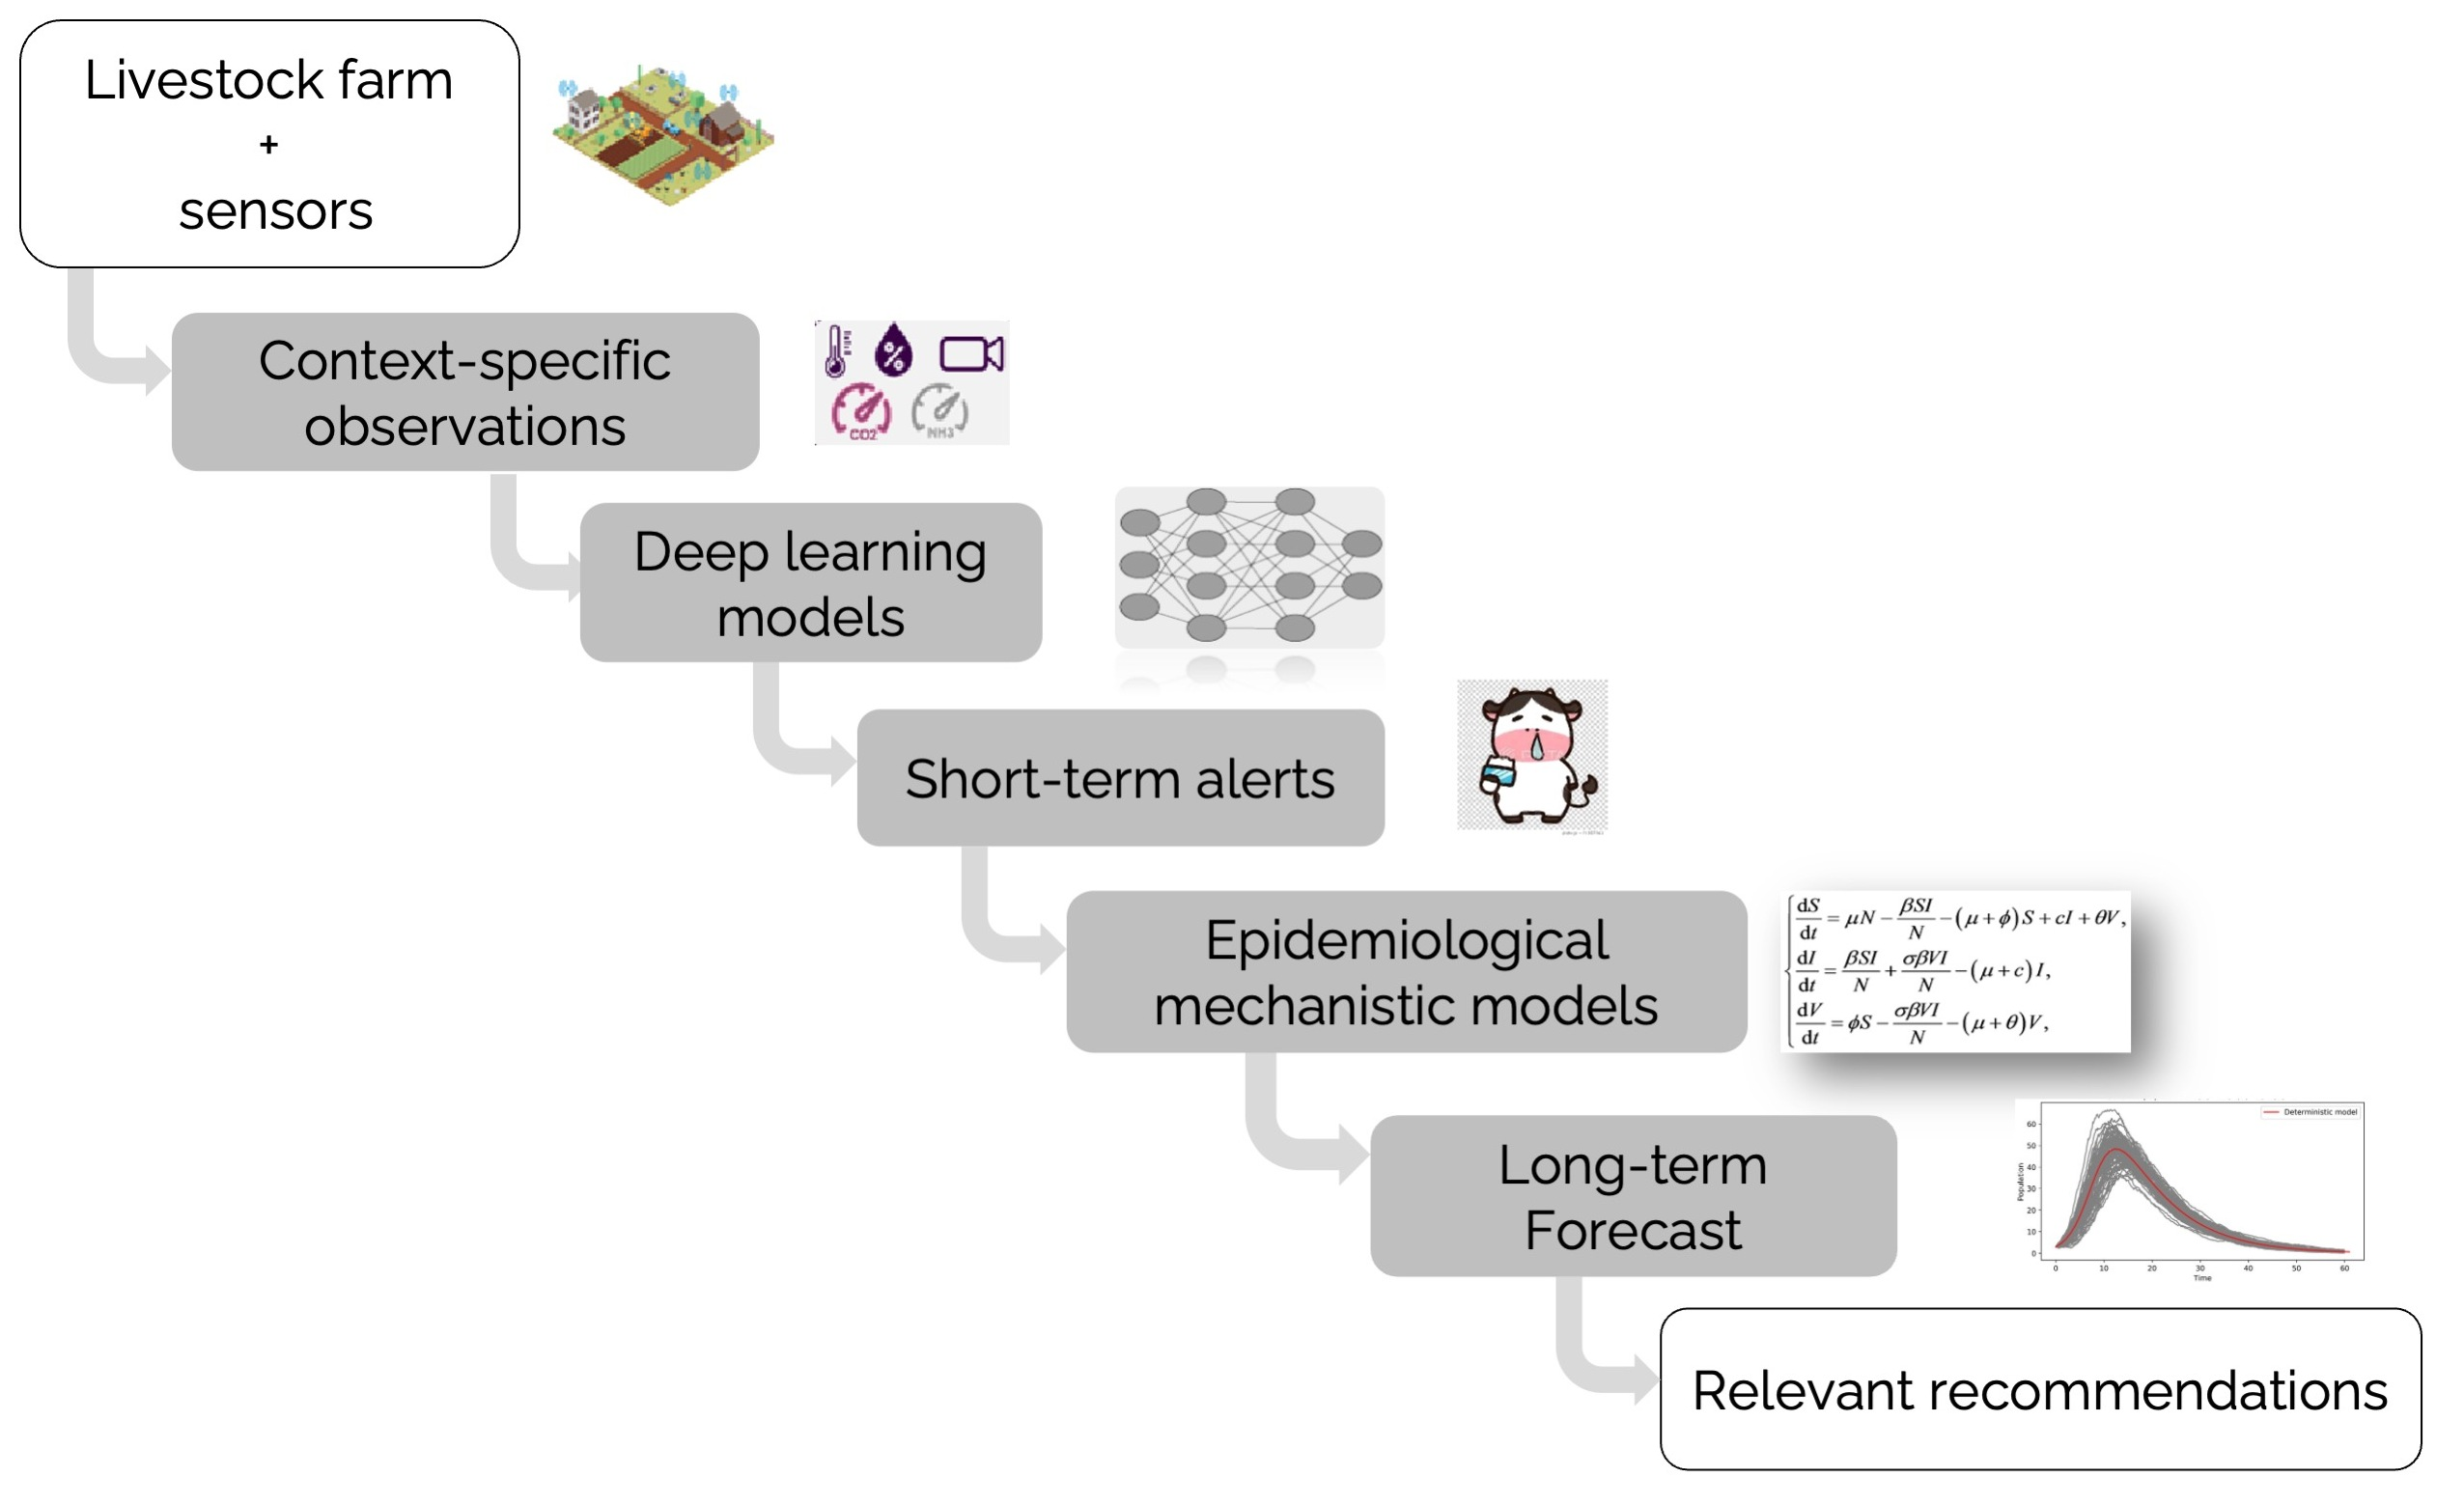
\includegraphics[width=\linewidth]{figures/chap1/chap1-outline.jpg}
  \caption{How can sensor observations be effectively employed to study infectious diseases and support informed decision-making?}
  \label{fig:chap1-outline}
\end{figure}
\newpage

Our primary hypothesis (Fig \ref{fig:chap1-outline}) posits that the optimal scientific approach to address contemporary quantitative challenges in animal health involves the integration of diverse artificial intelligence methodologies. In this thesis, we explore the complementarity between deep learning models and mechanistic epidemiological models. This integrative strategy leverages the extensive representation capabilities, multi-level analysis, and interdisciplinary expressivity of mechanistic epidemiological models while capitalizing on deep learning’s robust data-mining capabilities. This fusion aims to achieve better integration of real-world observational data (derived from sensors, farmers, and veterinarians) with disease predictions across multiple temporal scales—ranging from short-term (days) to medium and long-term (weeks or months).


\subsection{Use-case: Bovine Respiratory Diseases in young beef cattle sector}

Bovine Respiratory Disease (BRD) represents the foremost animal health concern in cattle feedlots, negatively impacting animal welfare, economic performance, and public health through excessive antimicrobial use \cite{s18082674}. BRD significantly reduces animal growth rates and productivity, resulting in increased veterinary and medicinal expenses, as well as higher mortality rates—averaging approximately 3\% 
\cite{Engler_Defoor_King_Gleghorn_2014}. It is also the primary reason antibiotics are administered in cattle production, affecting roughly 20\% of fattening cattle \cite{assie_exposure_2009}.

The aetiology of BRD is multifactorial (fig \ref{fig:chap1-BRDetiology}), arising from complex interactions among intrinsic and extrinsic factors. Intrinsically, animal susceptibility is influenced by breed, immunity, and simultaneous infection by multiple pathogens, notably Mannheimia haemolytica, Pasteurella multocida, and Bovine Respiratory Syncytial Virus (BRSV), whose interactions are not yet fully understood 
\cite{https://doi.org/10.1111/j.1751-0813.2003.tb13367.x, Duff2007}. Extrinsic risk factors—such as stressful transportation conditions, herd density, feed management, housing conditions, biosecurity protocols, and climatic conditions—also strongly influence disease occurrence and severity. Together, these intrinsic and extrinsic complexities severely limit the reliability of BRD prognosis, control strategies, and disease modelling.


\begin{figure}[h]
  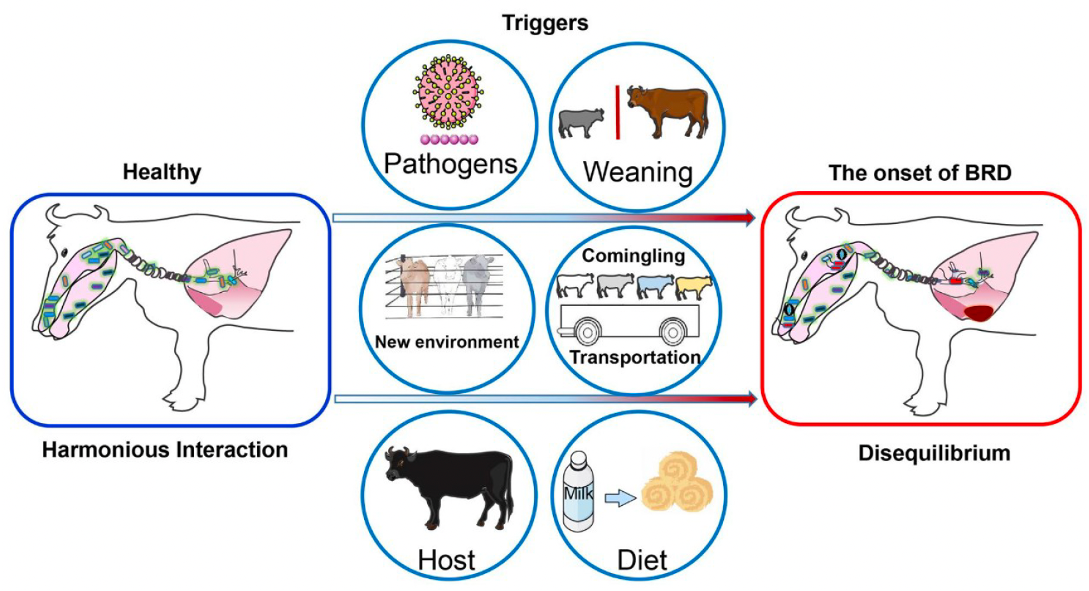
\includegraphics[width=\linewidth]{figures/chap1/BRD etiology.png}
  \caption{BRD etiology. From Jio-anmin et al., 2022. Burden in animal welfare, antimicrobial use and economic costs.}
  \label{fig:chap1-BRDetiology}
\end{figure}

Diagnosing BRD is particularly challenging due to non-specific clinical presentations such as cough, nasal discharge, hyperthermia, anorexia, lethargy, and impaired growth—symptoms overlapping with many other diseases \cite{https://doi.org/10.1111/j.1751-0813.2003.tb13367.x, GRIFFIN201057}. Traditional visual detection based on behavioural appraisal is limited, displaying low sensitivity (62\%) and specificity (approximately 63\%), thereby resulting in frequent misdiagnoses (false positives) or delays in detection \cite{doi:10.1177/104063870902100405, Duff2009}. Moreover, cattle often mask early clinical symptoms due to inherent prey behaviour, complicating timely and accurate identification of infected animals \cite{GRIFFIN201057}. Additionally, limited veterinary expertise in rural areas of France further exacerbates accurate detection.

Recent advances in precision livestock farming
\cite{Berckmans2014, Allain2014} have enabled continuous monitoring of animal health through sensor technologies such as accelerometers, microphones, thermometers, and cameras, measuring bio-signals indicative of BRD (e.g., body temperature, behavioural patterns, and respiratory sounds) \cite{Guatteo2015}. Timsit et al. (2011) previously demonstrated that about 73\% of hyperthermia episodes were associated with BRD, suggesting temperature-based monitoring's potential diagnostic utility \cite{timsit_early_2011}. More recently, Concordet et al. (2022) developed logistic regression models using sensor data (collar, pedometer, intra-ruminal bolus), achieving sensitivity and specificity rates of approximately 75\% and 76\%, respectively, capable of predicting BRD clinical signs up to 24 hours in advance \cite{Concordet2022}. Similarly, Ramezani et al. (2022) evaluated accelerometer-based ear-tag sensors detecting behavioural changes (activity, inactivity, rumination), demonstrating significant differences between healthy and diseased calves, although further validation in larger cohorts remains necessary \cite{ani12091093}.

Despite promising early detection results, most sensor-based studies remain limited by reliance on traditional machine learning models incapable of robust forecasting, hindering their predictive utility for scenarios that differ significantly from observed data. This limitation restricts their capacity to support evidence-based management and informed control interventions effectively, as complete observation of BRD dynamics in field conditions is ethically and practically unfeasible. One study even proposed that further studies with higher number of diseased animals are necessary to improve their performance. 

Complementary to sensor-based approaches, mechanistic epidemiological modelling has emerged as a promising solution to overcome observational limitations. Picault et al. (2022) \cite{picault_modelling_2022} conducted an in silico modelling study identifying potential sensor-based management strategies. However, these mechanistic models were primarily calibrated from existing veterinary literature rather than empirical sensor data, resulting in uncertainties regarding their practical and explanatory utility in real-world veterinary scenarios. Furthermore, such modelling often involves invasive and expensive sensor technologies, underscoring the necessity of exploring alternative, non-invasive, cost-effective sensor modalities (e.g., audio, video, image analysis) for broader deployment.

Addressing these critical limitations, this thesis, collaboratively developed by INRAE, Adventiel, and myself :), seeks to develop innovative artificial intelligence methodologies specifically tailored for BRD diagnostics and prognostics, yet adaptable to other livestock or plant epidemiological contexts. By integrating deep learning with mechanistic epidemiological modelling, this work explicitly aims to enhance the interpretability, accuracy, and predictive robustness of sensor-derived observations (see Fig \ref{fig:chap1-outline}). The resulting methodologies aims to minimize inappropriate antimicrobial usage, improve animal welfare, reduce economic losses, and support long-term, evidence-based decision-making in precision livestock farming.


% \textcolor{red}{dans les discussions pour le chapitre 1, il faudrait que j'indique que je notre sensibilité fait raccord avec ce qui est dit dans la littérature en utilisant uniquement les signes cliniques. Mais en quantifiant l'incertitude du modèle et celle contenue dans les données, on a pu améliorer la précision générale et en plus filtrer les observations considérée comme bruyantes.}


\subsection{Originality of this thesis}

\subsubsection*{A synergy of interdisciplinarity expertise}
% In this subsection, I want to explain the thesis CIFRE, with the mixture of domain expertise: epidemiological mechanistic modelling, statistical inference approaches, computer vision and deep learning, hardware and software engineering Mais également la collaboration avec les vétos. Préciser que c'est une thèse cifre (ce que peut apporter/ et les gains en retours pour adventiel: les côté applicatif, igepp (deep), Dynamo (mécaniste, inférence...). It is original to have as many different domain experts come together to work on one subject right ?

This doctoral project is structured under the CIFRE program ("Convention Industrielle de Formation par la Recherche"), an initiative established in France to foster collaboration between doctoral candidates, companies, and public research laboratories. The CIFRE framework encourages strong public-private partnerships, facilitating innovation that combines academic rigor with practical industry relevance.

In this thesis, such synergy is specifically realized through collaboration among distinct but complementary entities: Adventiel, INRAE (the French National Research Institute for Agriculture, Food, and Environment). Adventiel is a French company that specializes in digital solutions tailored specifically for the agricultural and agri-food sectors, providing services ranging from application development and artificial intelligence solutions to data science, software hosting, and comprehensive IT management. Their expertise and technological infrastructure, including advanced server configurations and data storage solutions, have substantially supported data collection and analysis during this research.

Complementarily, INRAE represents a world-leading public research institution dedicated to addressing critical global challenges such as climate change, biodiversity loss, and food security through the generation of scientific knowledge and innovation. INRAE's methodological approach emphasizes the integration of scientific insights from both animal and plant health domains. Indeed, one of INRAE's strategic research priorities has been to bridge methodological advances between these domains, a vision directly aligned with Adventiel's expanding R\&D activities. Leveraging this diverse expertise, the thesis incorporates critical methodological advances from each partner. From INRAE, particularly via the DYNAMO team within the BIOEPAR unit, this thesis benefits from the EMULSION framework. EMULSION \cite{EMULSION-ploscb2019}, is an innovative modelling tool combining knowledge representation and multi-agent systems to construct specialized epidemiological models. It includes a domain-specific language (DSL) tailored specifically for epidemiological modelling, which significantly facilitates interactions among interdisciplinary teams of biologists, veterinarians, and economists. Throughout this research, EMULSION's flexible and intuitive design greatly simplified adapting complex mechanistic models, enabling focused modifications even without extensive computational knowledge. Further, the BIOEPAR unit provided a solid foundational expertise in veterinary, epidemiological, immunological, and socio-economic aspects specifically related to bovine respiratory diseases (BRD). This included for instance the first mechanistic model developed for BRD within EMULSION, which served as a baseline for addressing key scientific questions in the present research.

In parallel, Adventiel contributed its extensive experience in developing deep learning solutions based on diverse data modalities (images, videos, and acoustic signals), aimed explicitly at creating indicators of animal welfare. Confidential deep learning architectures previously designed by Adventiel to analyse animal behaviour in video footage and detect anomalies in acoustic data provided methodological starting points. Additionally, Adventiel supplied essential hardware infrastructure and data management systems, which significantly streamlined data acquisition and analysis tasks throughout the thesis.

Finally, expertise from the Démécologie team of the IGEPP unit (INRAE) enriched the research by providing advanced statistical methodologies suited for inverse modelling, uncertainty quantification, and Bayesian inference. These methods are designed to analyse disruptions in epidemic dynamics at population scales, considering spatial and temporal variations, phenotypic plasticity, reproductive variability, and genetic factors. The team's statistical knowledge was instrumental in addressing several methodological and inferential challenges encountered in this thesis.

Thus, by combining these specialized competencies—ranging from computational modelling and deep learning to advanced statistical inference—this thesis tries to establish a robust interdisciplinary foundation, enabling innovative approaches to infectious disease diagnostics and management in livestock agriculture.

\subsubsection*{A multi-modal dataset for studying BRD in beef cattle farms}

During this thesis, an extensive observational dataset was collected as part of the Septime Project (Carnot France Futur Élevage), a collaborative initiative involving the BIOEPAR research unit (INRAE) and Idele (the French Livestock Institute). The objective of project SEPTIME is to integrate real-time sensor data with mechanistic epidemiological models, enabling theoretical disease progression scenarios to be continually updated and adjusted according to observed field conditions.

Data acquisition (Fig \ref{fig:chap1-DataCollection}) spanned two distinct periods aligned with the typical arrival schedules of cattle batches on farms: initially from January to June 2023, and subsequently from October 2023 to January 2024. These timeframes were specifically chosen based on evidence indicating that animals are at significantly elevated risk for Bovine Respiratory Disease (BRD) during the first few weeks following their arrival at new farms \cite{assie_exposure_2009}. Accordingly, sensor recordings and veterinary assessments commenced immediately upon the animals' arrival and continued consistently over the subsequent 30 days—a period recognized as crucial for early detection and effective management of BRD.

This dataset was specifically designed to facilitate detailed studies of Bovine Respiratory Disease (that is why is was done in collaboration with veterinarians working on the scientific question to determine immunologic markers of BRD) and comprised observations from nine beef fattening farms located across France. Within each farm, data was collected from up to three separate batches of cattle, each batch consisting of 5 to 12 animals. Approximately 78\% of these animals were of the Charolais breed, specifically chosen for its distinctive white fur that allows clearer visual detection of clinical symptoms.

To ensure comprehensive monitoring, multiple sensor modalities were installed and utilized systematically across these farms. Specifically, each farm was equipped with, One fixed video camera recording daily segments of 5 minutes every hour between 9 a.m. and 6 p.m., one microphone synchronized with video recordings to capture acoustic data concurrently and one environmental sensor continuously measuring ambient temperature, humidity, carbon dioxide ($CO_2$), and ammonia ($NH_3$) levels. Veterinary oversight played a pivotal role in enriching the dataset, with regular professional assessments conducted approximately every two days throughout the 30-day observation period following batch arrivals. Assessments could involved both clinical and biological examinations: clinical examinations included evaluations of animal behaviour and observable clinical signs, such as fatigue, ocular discharge, nasal discharge, and rectal temperature. Biological examinations entailed laboratory analyses of blood samples and polymerase chain reaction (PCR) testing of nasal swabs to detect the presence of pathogens within the animals’ upper respiratory tract.

\begin{figure}[h]
  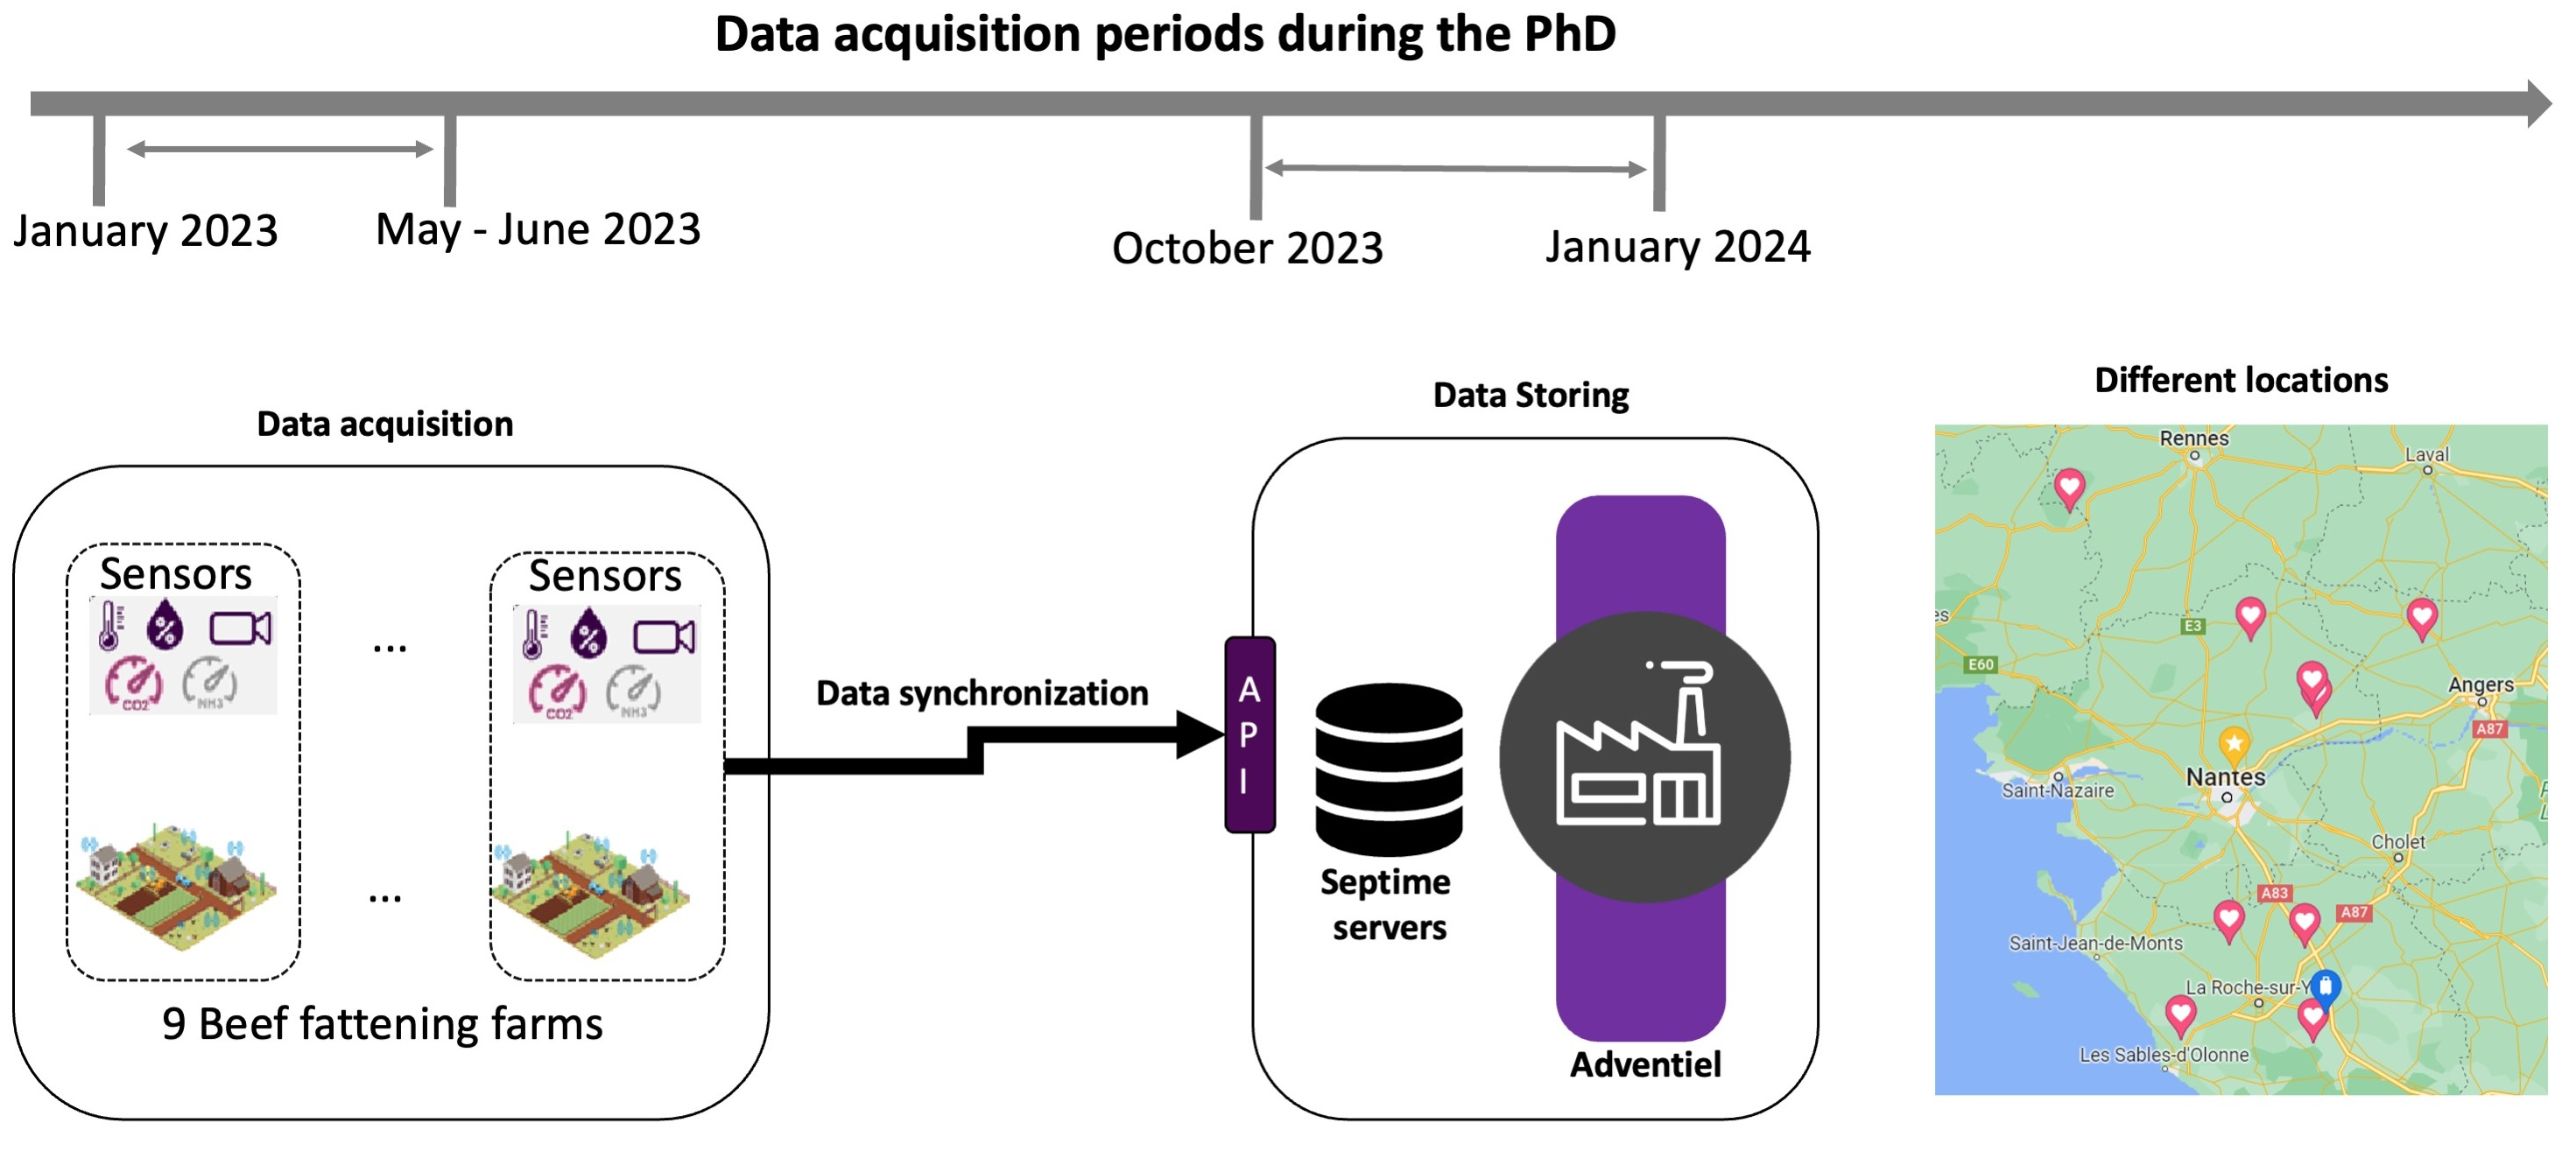
\includegraphics[width=\linewidth]{figures/chap1/data collection.jpg}
  \caption{Overview of data acquisition protocol put in place for bovine respiratory disease monitoring}
  \label{fig:chap1-DataCollection}
\end{figure}

Additionally, lung ultrasound scans were periodically conducted as a complementary diagnostic method. These ultrasound examinations occurred on scheduled days (day 0, day 5, day 14, day 21, and day 28), depending on veterinarian availability. Ultrasound recordings provided detailed visual assessments of lung condition, enhancing the dataset’s diagnostic depth. In parallel with the on-farm data collection, considerable effort was devoted to configuring reliable communication and secure data transfer between installed sensors and Adventiel's remote data storage servers. This integration was to ensured that collected sensor observations was systematically organized, stored, and made readily accessible for subsequent statistical and computational analyses.

Collectively, this dataset—comprising synchronized multimodal sensor recordings, veterinarian clinical and biological assessments, and ultrasound imaging, has provided a solid empirical foundation that simultaneously addresses fundamental research questions and practical agricultural objectives. In the next subsection, we clearly explain how we proceeded to tackle our scientific question, which sensor observation, which first questions and the potential contributions we bring through our work.

%[\textcolor{red}{I need to give me factual details on the current state of data: storage space, left to do (discussion). gotta Check and verify with Maud's documents for more detail}]
 

\subsubsection*{About the methodological approach and contributions}

The central methodological ambition guiding this thesis is to demonstrate how coupling deep learning methods with mechanistic epidemiological modelling can effectively leverage sensor-derived observations to enhance animal health through the the study and the control of infectious disease in livestock farming. This integrative approach seeks to address the inherent uncertainties and practical limitations associated with sensor technologies (particularly when observations are sparse, noisy and incomplete) by employing powerful data processing methods and robust interdisciplinary theoretical knowledge into a novel modelling approach. We chose to test and assess our modelling approach to study and control BRD, as it is currently ongoing and challenging problem to tackle that has lots negative impacts (antimicrobial usage, public health safety, animal welfare, farmer wellbeing, etc)

Our investigation unfolds methodologically across three interlinked chapters, each addressing a distinct yet complementary facet of the overarching scientific inquiry. The journey begins in Chapter 2, where we set foundational structures to independently examine the feasibility and robustness of both deep learning and mechanistic models in the specific context of Bovine Respiratory Disease (BRD). We ask: "To what extent can deep learning reliably automate short-term diagnosis using limited and context-specific sensor data, such as lung ultrasound videos?" Using a tailored CNN-RNN architecture, we demonstrate the feasibility of automated diagnosis from limited observational data, achieving approximately 72\% diagnostic accuracy on lung ultrasound videos collected in real-world farm conditions. Concurrently, we explore the second fundamental question: "Can empirical veterinary observations reliably be used to parametrize a mechanistic epidemiological model to provide long-term BRD prognosis?" Here, we successfully parametrize a stochastic mechanistic model using veterinary assessments, highlighting its potential for reconstructing disease dynamics over longer time horizons despite inherent uncertainties in sparse observations. These findings collectively provide an empirical baseline for further integrated analyses and constitute original contributions through the creation of a unique, annotated dataset of lung ultrasound observations, critical for future research. Inspired by the "Mixture of Experts" (MoE) concept, our methodological approach explicitly acknowledges and leverages the distinct strengths of each modelling approach. We strategically delineate diagnostic tasks, which are handled by deep learning due to their robust semantic feature extraction capabilities, from prognostic tasks, which mechanistic epidemiological models perform effectively due to their capacity for long-term dynamic prediction grounded in theoretical epidemiological principles. This systematic division of expertise ensures that each methodological component is utilized in the domain where it is most effective. Additionally, the unique annotated lung ultrasound dataset we have collected and labelled could represent a contribution and an invaluable resource for future research.


Building upon this foundation, Chapter 3 delves deeper into methodological complexities by explicitly addressing scenarios involving multiple plausible pathogen-specific mechanistic models. The central inquiry of this chapter is twofold: first, "To what extent can we reliably differentiate between multiple pathogen-specific mechanistic models of BRD solely based on symptomatic observations?", and second, "Does the identification of the correct pathogen-specific model significantly improve practical decision-making outcomes?". The necessity for multiple, specialized prognostic experts can be illustrated through a familiar medical analogy: when a patient experiences symptoms, they first consult a general physician who must then determine which specialist—whether a cardiologist, neurologist, or pulmonologist—should handle the diagnosis and subsequent treatment. Similarly, accurate long-term prognosis of BRD requires identifying the correct pathogen-specific mechanistic model (or "specialist") based on observed diagnosis to ensure that the resulting recommendations align effectively with disease-specific management strategies. To tackle these critical questions, we propose a novel methodological approach employing Approximate Bayesian Computation coupled with multinomial logistic regression, successfully distinguishing pathogen-specific models (BRSV, Mh, and Mb) with approximately 93\% accuracy based solely on observed symptomatic trajectories. Crucially, we further integrate these pathogen-informed predictions into a detailed bio-economic framework, demonstrating tangible improvements in farm-level decision-making outcomes—including a remarkable 44\% reduction in antimicrobial use and a modest but meaningful increase in profitability. These results underscore the importance of rigorously linking epidemiological modelling with actionable decision-making, highlighting practical implications that extend beyond academic curiosity.

The narrative culminates in Chapter 4, where the methodological integration becomes explicit and adaptive. This final chapter poses two pivotal questions: "Can automated short-term diagnostics derived from limited sensor observations effectively specify a mechanistic epidemiological model for robust long-term disease prognosis?" and critically, "How can intrinsic uncertainties inherent in noisy sensor-derived diagnostic data be explicitly quantified and incorporated into prognostic predictions?" To address these questions, we present an innovative Bayesian Deep Mechanistic (BDM) approach, a structured hybrid model that explicitly integrates deep learning-based diagnostic predictions from lung ultrasound (LUS) video data with a mechanistic epidemiological model. By employing Monte Carlo Dropout (MCD), we systematically quantify and manage uncertainties inherent in the noisy, limited sensor data—effectively enhancing diagnostic accuracy from an initial 39\% error to a robust 27.2\% relative root mean squared error (RRMSE). This explicit uncertainty quantification not only substantially improves the robustness and reliability of short-term automated diagnostics but critically also enhances long-term disease forecasts. The dual methodological strategies explored, uncertainty-based filtering and uncertainty-weighted inference, demonstrate how explicitly incorporating uncertainties into mechanistic models significantly closes the predictive accuracy gap between purely automated sensor-based forecasts and expert-driven prognostics, thus providing a robust and practical decision-support tool for livestock management.

General discussion - The final section synthesizes the findings across all chapters, critically evaluating the methodological approaches, their strengths and limitations, and the broader implications of the results. Recommendations for future research and applications are also discussed, highlighting the potential for scalability and interdisciplinary adaptation. Across these chapters, the contributions of this thesis converge into a comprehensive methodological framework characterized by automated diagnostics, robust prognostics, clear model differentiation strategies, explicit uncertainty quantification, and practical decision-making integration. The modularity and flexibility of the approach developed here encourage its broader applicability across diverse epidemiological contexts, inviting domain experts, from veterinarians and deep learning specialists to mechanistic modellers, to further adapt and refine these methodologies. 

% Les fronts de science traités pendant cette thèse seront donc (i) le développement d'algorithmes d'apprentissage profond spatio-temporelle et/ou ensembliste pour la construction de descripteurs santé [Mahmud et al 2021], (ii) l'étude de la fiabilité de ces descripteurs pour le couplage au modèle mécaniste (e.g. biais, variance, cohérence) et enfin (iii) l'étude des capacités prédictives des modèles mécanistes informés par de tels indicateurs sur des horizons épidémiques longs.

